\chapter{Theory and Terminology}
\label{cha:solutioni}
In this chapter, we are going to discuss the theory and terminology used in this work.
Representing words in a vectorial form is an essential element in natural language processing. We have used a number of algorithms for getting such vector representations. In this chapter, we will briefly explain the background needed to understand those algorithms.
\section{Machine learning Algorithms at our disposal}

\subsection{Principle Component Analysis(PCA)}
Principal component analysis(PCA) is a very important tool in data analysis. It is a simple, non-parametric, mathematical tool that can be used in variety of fields where large amount of data is being generated. Importance of PCA can be understood from the fact that it can be very efficiently used in extracting information from a vague data set and is highly useful in dimensionality reduction. \\\\
In the real world settings, the data set which needs to be analyzed is generally very obscure and can be very high dimensional. This data usually have various outliers, errors or redundancy. Therefore preprocessing is vital before analyzing it. Even after preprocessing, it is difficult to figure out what this data is representing as it might be present in a high dimensional space. This makes it hard, not only to visualize but also to apply machine learning algorithms such as clustering or classification. Thus making "dimensionality reduction", very important in this data-driven world.\\ 
Data that is produced by various processes generally rely on a number of parameters but not all of these parameters are important for analyzing this data efficiently. An example of such a scenario is that if we have a naive experiment setting in which we do not know the underlying dynamics of the experiment. Then it is difficult to express this experiment as a function of some parameters.\\\\
"Principal Component Analysis(PCA)" helps in reducing a complex data set to a lower dimensional space thus revealing the hidden, dynamics. It helps in getting the most meaningful basis to re-express any noisy data set. The general consideration is that each data sample is represented in \textit{m}-dimensional space and all the vectors in such a space are in a linear combination of a set of unit basis vectors. PCA tries to explore some other basis, which best "re-expresses" the data and is a \textit{"linear"} combination of original basis. The main point to notice here is that PCA makes an assumption of \textbf{linearity}, thus making a limitation of re-expressing the data only as a linear combination of its basis vectors. Let $\mathbf{Y}$ is the re-expressed data set of the original data set, $\mathbf{X}$ and let $\mathbf{P}$ be the transformation matrix used in such a transformation. Then we can represent this basis transformation by the equation \ref{eq:pca}.
\begin{equation}\label{eq:pca}
\mathbf{PX = Y} 
\end{equation}
%\subsubsection{When to use PCA}
To understand how PCA finds the best solution for re-expressing $\mathbf{X}$ and for selecting a good choice for the basis transformation $\mathbf{P}$, one should understand what features, $\mathbf{Y}$ should have. When the data set is collected, it might contain: \textit{noise} and \textit{redundancy}.
\begin{enumerate}
	\item{Noise:} Noise should be as low as possible in a data set. A metrics to measure noise is \textit{Signal to noise ratio(SNR)} given by:
	\begin{equation}
	\mathit{SNR} = \dfrac{\sigma^2_{signal}}{\sigma^2_{noise}}
	\end{equation}
	where: $\sigma$ represents standard deviation and $\sigma^2$ represents the covariance.
	\item{Redundancy:} 
	Redundancy is also very important to deal with when it comes to dimensionality reduction. It is important to eliminate those dimensions which express the redundant information. This helps in eliminating dimensions which are not crucial without loosing information. 
\end{enumerate}
\subsubsection{Solving PCA with eigen value decomposition}
\subsubsection{Covariance Matrix}
Covariance matrix represents the strength of corelation between data points. If the data points are correlated in some way, then the covariance between these points will be nonzero and vice versa. While analyzing the covariance, the exact value is not as important as the sign of the values. If the value is positive, then this mean that the data points in question are increasing together. On the another hand, if the value is negative then this mean that when one increases, other one decreases. If the value is zero, then it means that both are independent of each other.\\
\begin{equation}
\sigma^2_A = \langle \mathit{a_ia_i} \rangle_i
\end{equation}
\begin{equation}
\sigma^2_B = \langle \mathit{b_ib_i} \rangle_i\\
\end{equation}
Covariance of $\mathit{A}$ and $\mathit{B}$ will be given by:
\begin{equation}
\sigma^2_{AB} = \langle \mathit{a_ib_i} \rangle_i
\end{equation}
\begin{equation}
\sigma^2_{AB} = \langle \mathit{(A-\mu_A)(B-\mu_B)} \rangle_i
\end{equation}
where: $\mu$ is the mean\\
The set of data points $\textbf{X}$, can be represented as row vectors matrix. In such a case, covariance, $\mathbf{S_X}$ can be calculated using:
\begin{center}
	$\mathbf{X} = [\mathbf{x}_1,\mathbf{x}_2 ... \mathbf{x}_n]^T$\\
\end{center}
\begin{center}
	$\mathbf{S_X} = \frac{1}{n-1}\mathbf{XX}^T$
\end{center}	
The main goal here is to minimize the redundancy, which is possible if the covariance between data points can be reduced. From interpretation of figure \ref{fig:redundancy}, to remove redundancy, the covariances between different data points should be zero. Let the "optimized covariance matrix" be $\mathbf{S_Y}$, then this matrix satisfies the above condition only when it is a diagonal matrix. 
\begin{figure}[H]
	\centering
	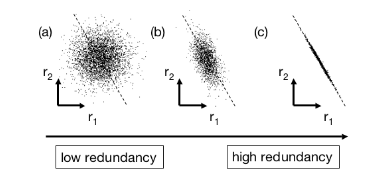
\includegraphics[width=10cm,height=12cm,keepaspectratio]{files/redundancy.png}
	\caption{A spectrum of possible redundancies in data for \textit{r1} and \textit{r2} (\cite{shlens2014tutorial})}
	\label{fig:redundancy}
\end{figure}
There are numerous ways to "diagonalize the covariance matrix" or to reduce noise and redundancy, but one of the easiest method is offered by PCA. The solution to PCA is based on \textit{eigenvectors} computation. 
The goal of PCA is to find an orthogonal matrix $\mathbf{P}$ where $\mathbf{Y = PX}$ such that $\mathbf{S_Y}$, in equation \ref{eq:diag}, is a diagonal matrix. \\
\begin{equation}\label{eq:diag}
\mathbf{S_Y = \frac{1}{(n-1)}YY^T}
\end{equation}
The rows of this orthogonal matrix, $\mathbf{P}$, are the principal components of $\mathbf{X}$. It can be illustrated as follows: $\mathbf{S_Y}$ can be written in terms of $\mathbf{P}$\\
\begin{equation} \label{eq:split}
\begin{split}
\mathbf{S_Y} & = \frac{1}{(n-1)}\mathbf{YY^T}\\
& = \frac{1}{(n-1)}\mathbf{(PX)(PX)^T}\\
& = \frac{1}{(n-1)}\mathbf{P(XX^T)P^T}\\
\mathbf{S_Y} &= \frac{1}{(n-1)}\mathbf{PAP^T}\\
\end{split}
\end{equation}
Where: $\mathbf{A}\equiv\mathbf{XX^T}$ and $\mathbf{A}$ is a symmetric matrix. Since a symmetric matrix can be diagonalized by a matrix, $\mathbf{D}$ of its orthogonal eigenvectors, $\mathbf{E}$. Hence:
\begin{center}
	$\mathbf{A} = \mathbf{EDE^T}$
\end{center}
The matrix $\mathbf{P}$ is selected such that each row in $\mathbf{P}$ represented by $\mathbf{p_i}$ is an eigenvector of $\mathbf{XX^T}$. In other words, the principal components of $\mathbf{X}$ are eigenvectors of $\mathbf{XX^T}$.   
\subsubsection{Steps in PCA}
In practice, PCA has very simple steps:
\begin{enumerate}
	\item We have a dataset, represented by $\mathit{m\times n}$ matrix, where $\mathit{m}$ is number of dimensions and $\mathit{n}$ is number of data items in the set. In other terms, the matrix is a data matrix.
	\item Compute the zero mean matrix for the data matrix.
	\item Calculate the eigenvalues and eigenvectors of the covariance matrix of the data set.
\end{enumerate}
As mentioned earlier in this section, one important usage of PCA is for \textit{dimensionality reduction}. The eigenvectors represent the principal components of the dataset. The greatest variance lies in the first principal component and so on.\\
If the dimensionality is to be reduced from $\mathit{m}$-components to $\mathit{k}$-components, then we can find the largest variance associated with the data in the first $\mathit{k}$-components. In this way, it can be made certain that loss of information is minimum and also important information is not lost in the process.
The calculations can be understood from the following equations:
\begin{center}
	$\mathbf{X} =\mathbf{(EE^T)X} $
\end{center}
\begin{center}
	$\mathbf{X = EH}$
\end{center}
\begin{center}
	If $1\leq k< m$:
\end{center}
\begin{center}
	$\mathbf{x_i}\approx \sum_{j=1}^{k}\mathbf{e}_jh_{ji} = \mathbf{y_i}$
\end{center}
Thus $\mathbf{Y}$ is the new data matrix with reduced dimensions of $\mathit{k\times n}$
\subsubsection{Limitations and Assumptions of PCA}
It is also important to understand the instances where PCA does not give the expected results. Some of them are as follows:
\begin{enumerate}
	\item \textbf{Linearity:}
	PCA makes an assumption that the data is linearly correlated. With this assumption, PCA gets limited to re-express data only as a linear combination of the basis vectors. Hence if the data is non linear then PCA will not work as expected. In such cases, Kernel PCA can be used.
	\item \textbf{Means and variance are needed:}
	PCA assumes that only mean and variance are needed to describe the distribution. This assumption works only when data is obtained from a Gaussian distribution. But when data is not Gaussian then these assumptions does not hold true and one won't get the desired results. 
	\item \textbf{PCA always finds orthogonal principal components:}
	Sometimes, we need to non-orthogonal principal components to represent the data set. But with PCA, the components of the data set are always orthogonal and hence it won't be useful.
\end{enumerate}

\subsection{Random Projection}
Some times the data set, that we need to analyze, is in a very high dimensional space such that it becomes very expensive to compute principal components directly. \cite{bingham2001random} illustrated that projecting a very high dimensional data on a random lower-dimensional subspace also results in a preserving important information in the data. Theoretical results cited by \cite{bingham2001random} indicate that the method preserves distances quite nicely. They also showed experimentally that using a sparse random matrix helps avoiding additional computations.\\\\
In such a random projection approach, the high dimensional data of dimension $d$ is projected to a lower-dimensional space of dimension $k$, where $(k \ll d)$, using a random $ k \times d$ matrix, $\mathbf{R_{k\times d}}$.
\begin{equation}
	 \mathbf{X}_{k\times N} = \mathbf{R}_{k\times d} \mathbf{X}_{d\times N}
\end{equation}
The random projection is based on the idea of Johnson-Lindenstrauss lemma proposed by \cite{johnson1984extensions}. In the lemma, it has been proposed that if points in a vector space are projected onto a randomly selected subspace of suitably high dimension, then the distances between the points are approximately preserved. But one can argue that matrix $ \mathbf{R} $ should be orthogonal, which will not be the case always. Orthogonalization of $ \mathbf{R} $ can be expensive and defeats the whole purpose. But it has been proved by Hecht-Nielsen that in a high dimensional space, there are many unit vectors which are almost orthogonal. Hence such a matrix can be used without losing so much.\\
\cite{dasgupta2000experiments} has also stated many benefits of using a Random projections over PCA. As discussed in limitations of PCA, that it can be used on the data with Gaussian distributions but in case of a mixture of $ \mathit{k}$ Gaussian, it cannot reduce dimensionality below $\Omega(k) $. When using, Random projections this can be done in $\mathcal{O}(log(k))$. But the performance of PCA is far better when the projection dimension is less than $log(k)$.\\\\
The key point of interest is how to choose the random matrix $ \mathbf{R} $ so that $ \mathbf{R^T R} $ be an approximate identity matrix. There have been two good approaches for this choice. The first being \textit{Gaussian Random Projection}, where each element is obtained from a distribution of type $\mathcal{N}(0, \frac{1}{n_{components}})$. The second alternative is \textit{Sparse Random Projection}, which according to \cite{achlioptas2001database} and \cite{li2006very} can be used instead of using a Gaussian. Here a very simple projection of the type presented below can also be used instead.
\begin{center}
	$\mathit{r_{ij}} = \left\{ \begin{array}{c c l} -\sqrt{\frac{s}{n_{\text{components}}}} & & 1 / 2s\\\\ 0  && 1 - 1 / s \\\\ +\sqrt{\frac{s}{n_{\text{components}}}} & & 1 / 2s\\ \end{array} \right.$
\end{center}
where:
\begin{center}
	$\mathit{s} =\frac{1}{density}$ and 
	$\mathit{density} = 1 / \sqrt{n_{\text{features}}}$
\end{center}
From the results, presented by \cite{bingham2001random}, it can be inferred that the random projection preserves the similarities of the data vectors quite well even when the data is projected to moderate numbers of dimensions. This method of projection is thus faster to compute and helpful when we cannot compute PCA. 
\subsection{Kernel Function}
In machine learning, the main goal can be summed up to predict a "function" through which we can represent not only the given data set but also the future data set. When given a set of data, it is not an herculean task to detect linear relations with model fitting. The main problem arises when the relation between the data set is not linear. Such a data set can be said to be linearly separable in an unknown higher dimension. In other words the data set can be mapped to a higher dimensional space where the relation between the data points becomes "linear". Thereafter the linear regression can be easily applied in that dimensional space.\\\\
This is a theoretical approach which becomes very difficult to implement because of the fact that the dimensional space, where the data relation becomes linear, is unknown. The solution for this problem is known as \texttt{Kernel Trick}.
\begin{figure}[H]
	\centering
	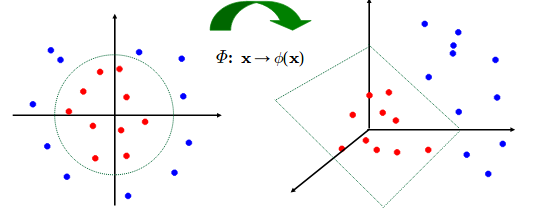
\includegraphics[width=10cm,height=12cm,keepaspectratio]{files/kernel.png}
	\caption{Transformation from one space to another using a Kernel fucntion $\phi$ (\cite{lecKernel})}
	\label{fig:kernel}
\end{figure}
The kernel trick is a mathematical tool which can be applied to any algorithm which consists of a dot product between two vectors. Kernel trick states that to compute the dot products of vectors in the higher dimensional space, a kernel function can be used directly using the lower dimensional vectors. Therefore every dot product can be replaced by this kernel function. A \textit{Kernel function}, can thus be defined as a function that takes as inputs vectors in the original space and returns the dot product of the vectors in the feature space. The feature space is usually a higher dimensional space.\\
\begin{equation}
\phi \, : \, {\rm I\!R}^n \to {\rm I\!R}^m
\end{equation}
where: m > n\\
\begin{equation}
k(\mathbf x, \mathbf y) = \phi(\mathbf x)^T \phi(\mathbf y) 
\end{equation}
\subsubsection{Which functions can act as Kernel functions?}
In order for a function to be a valid \texttt{Kernel function}, it should fulfill the \texttt{"Mercer's theorum"}. According to the Mercers' theorem, every positive definite symmetric function can be seen as a kernel function. Here a positive definite symmetric functions correspond to a "positive definite symmetric Gram matrix" which can be understood as a matrix which has all positive eigenvalues. Therefore a function which fulfill these conditions can be refereed as \textit{kernel function}.\\\\
There are many choices of the kernel function, $\mathit{k}$,which are as follows:\\
\begin{enumerate}
	\item \textbf{Linear Kernel:}
	It is the simplest type of kernel function. It can be denoted as follows:
	\begin{center}
		$\phi : \mathbf{x} \rightarrow \phi(\mathbf{x})$
	\end{center}
	\begin{center}
		where $\phi(\mathbf{x})$ is $\mathbf{x}$ itself
	\end{center}
	Thus a linear kernel can be of form:
	\begin{equation}
	k(\mathbf{x},\mathbf{y}) = (\mathbf{x}^T \mathbf{y} +1)
	\end{equation}
	Linear kernel finds its usage mostly in text classification tasks. The most important usage of this Kernel is in SVM as training a SVM with a linear kernel is much faster as compared to other kernels.
	\item \textbf{Polynomial Kernel:} 
	A polynomial kernel is a function which maps the input space into a non-linear space represented by a polynomial function. It can be denoted as follows:
	\begin{equation}
	k(\mathbf{x},\mathbf{y}) = (\mathbf{x}^T \mathbf{y} +1)^p
	\end{equation}
	\begin{center}
		where: $p$ is the degree of the polynomial.
	\end{center}
	\item \textbf{Gaussian Kernel}\\
	Also known as radial basis function kernel (RBF), it is one of the most powerful kernels. 
	Since the value of RBF kernel decreases with distance and ranges between 0 and 1 (when x = $x'$), it can be used as a similarity measure.
	\begin{equation}
	k(\mathbf{x},\mathbf{y})=\exp\left(-\frac{\|\mathbf{x}-\mathbf{y}\|^{2}}{\sigma^{2}}\right) 
	\end{equation}
	The Gaussian RBF kernel is very popular and makes a good default kernel as the feature space of this kernel has an infinite number of dimensions.
\end{enumerate}
\subsection{Kernel PCA}
Kernel Principle Component Analysis is the nonlinear form of PCA, which allows to generalize standard PCA to nonlinear dimensionality reduction. In other words, it can be referred as a non-linear dimensionality reduction technique through the use of kernel function. 
\begin{figure}
	\centering
	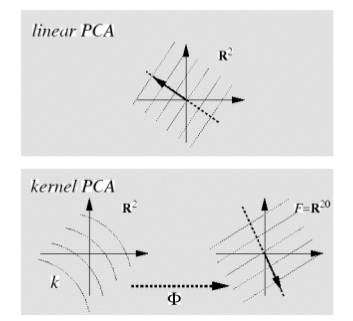
\includegraphics[width=10cm,height=12cm,keepaspectratio]{files/kernelPCA.png}
	\caption{ Kernel PCA: A nonlinear kernel function $\kappa$is used instead of the standard dot product. It implicitly perform PCA in a  possibly high-dimensional space $ F $ which is  nonlinearly related to input space. (\cite{scholkopf1997kernel})}
	\label{fig:kpca}
\end{figure}
\cite{scholkopf1997kernel} have shown that the generalization of PCA for non-linear data can be done via a kernel function.
\begin{equation}
covar = \dfrac{1}{N}\sum_{i=1}^{N}\phi(\mathbf{x}_i)\phi(\mathbf{x}_i^T)
\end{equation}
The covariance matrix in the higher dimensional space is not calculated explicitly but with using a kernel function such that: 
\begin{equation}
\kappa(\mathbf{x},\mathbf{y}) = \mathbf{\langle\phi(x),\phi(y)\rangle} =  \mathbf{\phi(x)^{T}\phi(y)}
\end{equation}
\begin{center}
	where: $\phi :{\rm I\!R}^d \rightarrow {\rm I\!R}^N $\\
	$\kappa$ is kernel function eg: radial basis function.
\end{center}
However, it is not guaranteed that the kernel matrix is centered, therefore to achieve the centered kernel matrix, \cite{scholkopf1998nonlinear} proposed:
\begin{equation}
\mathbf{\tilde{K} = K -I_NK-KI_N+I_NKI_N}
\end{equation} 
\begin{center}
	where: $\mathbf{1_N}$ is a $N\times N$ matrix with values equal to $\dfrac{1}{N}$
\end{center}
The standard steps of kernel PCA dimensionality reduction can be summarized as discussed by \cite{wang2012kernel}:
\begin{algorithm}[H]
	\caption{Kernel PCA}\label{kernelpca}
	\begin{algorithmic}[1]
		\State Construct the kernel matrix $\mathbf{K}$ from the training data set $\{\mathit{x_i}\}$ where $\mathbf{K_{ij}} = \mathit{\kappa(\mathbf{x}_i,\mathbf{x}_j)}$.
		\State Compute the kernel centered matrix  $\mathbf{\tilde{K}}$
		\State Solve $ \mathbf{\tilde{K} a}_\mathit{k} = \lambda_k N \mathbf{a}_\mathit{k}$ for the value of $\mathbf{a}_\mathit{i}$
		\State Compute  the  kernel  principal  components $y_k(\mathbf{x}) = \sum_{i=1}^{N} a_{k,i}\kappa(\mathbf{x,x}_i)$
	\end{algorithmic}
\end{algorithm}
\cite{scholkopf1997kernel} have also stated some advantages of using \textit{Kernel PCA}, for example, nonlinear principal components afforded better recognition rates than the linear ones. Another advantage is that better performance can be achieved for the nonlinear components by using more components which is not the case in the linear components. This can be used for applications such as feature extraction and data classification. 
\subsection{Artificial Neural networks and Deep Learning}
Artificial Neural Network or ANN is a term inspired by the sophisticated functionality of the human brain. In mathematical terms one might consider artificial neural networks as \textit{"universal function approximators"}.
A neural network is a collection of connected units called artificial neurons. The nodes takes the input data and perform some simple operations on the data. The output at each node is called its activation. This output can act as the input for the other nodes. Each link is also associated with a weight. This weight is assigned on the basis of its relative importance to the other inputs. A simple neuron can be represented by the \ref{fig:neuron}\\
\begin{figure}[H]
	\centering
	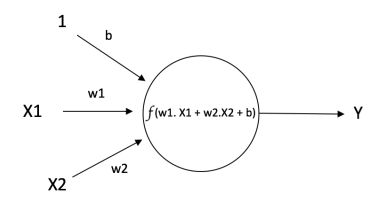
\includegraphics[width=10cm,height=12cm,keepaspectratio]{files/neuron.png}
	\caption{A single neuron with output $Y =f(w1.X1+w2.X2+b)$ (\cite{neuron})}
	\label{fig:neuron}
\end{figure}
The main aim of a neural network is to approximate some function $\mathit{f'}$. To attain such a goal, they define a mapping, $\mathbf{y} = f(\mathbf{x;w})$ and try to learn the parameters, $\mathbf{w}$, which makes the best approximation for the function $\mathit{f'}$. 
A non-linear transformation with function "$\phi$" can be applied on input $\mathbf{x}$ to extend linear models to represent nonlinear models. 
\begin{equation}
\mathbf{y} = f(\mathbf{x;w,\theta)} = \phi(\mathbf{x;w})^T \mathbf{\theta}
\end{equation}
Alternatively, \textbf{kernel trick} can also be used for such transformation. The advantage of using the neural networks is that the transformation function $\phi$ is not hard coded but can be learned and thus eliminating the need of manually engineer the function $\phi$. 	
\subsubsection{Types of Artificial Neural Networks}
\begin{enumerate}
	\item \textbf{Feedforward ANN:} 
	As the name indicates, a model is known as \textit{feed-forward neural network} when the information flows in the forward direction through a function, $f$, being evaluated from $\mathbf{x}$ through the intermediate computations and finally to the output $\mathbf{y}$. Such networks are also known as multilayer perceptrons(MLP). \\
	\begin{figure}[H]
		\centering
		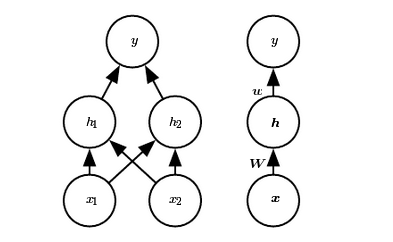
\includegraphics[width=10cm,height=12cm,keepaspectratio]{files/feedForward.png}
		\caption{Forward Neural Network (\cite{Goodfellow-et-al-2016})}
		\label{fig:fnn}
	\end{figure}
	\item \textbf{FeedBack ANN}
	In these neural networks, a feedback connection is present through which the outputs of the model are fed back into itself thus taking the previous time stamp's results into account. Such neural networks are also known as \textit{Recursive or Recurrent Neural Network}.
	\begin{figure}[H]
		\centering
		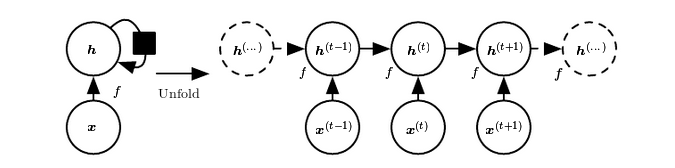
\includegraphics[width=10cm,height=12cm,keepaspectratio]{files/recurrentNN.png}
		\caption{A recurrent network with no outputs. This recurrent network just processes information from the input $\mathbf{x}$ by incorporating it into the state $\mathbf{h}$ that is passed forward through time$\mathbf{t}$. (Left) Circuit diagram. The black square indicates a delay of a single time step. (Right) The same network seen as an unfolded computational graph, where each node is now associated with one particular time instance (\cite{Goodfellow-et-al-2016})}
		\label{fig:fnn}
	\end{figure}
\end{enumerate}
\subsubsection{Design paradigms of a Neural Networks}
\begin{enumerate}
	\item \textbf{Activation function}
	The function, $f$ in figure \ref{fig:neuron} is a non-linear function and referred as an activation function. The purpose of such a function is to introduce non-linearity in the output of the neuron. There are various activation functions that can be used, some of them are represented in figure, \ref{fig:act}
	\begin{figure}[H]
		\centering
		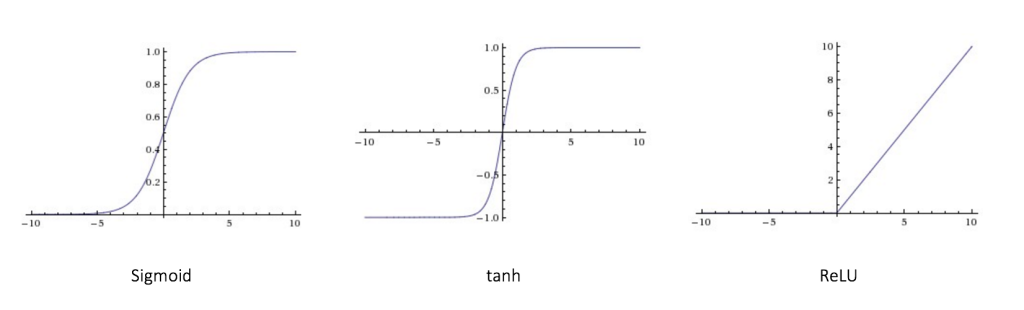
\includegraphics[width=15cm,height=25cm,keepaspectratio]{files/act.png}
		\caption{Popular activation functions generally used. (\cite{neuron})}
		\label{fig:act}
	\end{figure}
	Non linear activation functions are usually preferred because if a linear function is used then neural networks are as effective as a network with only one layer, regardless of how complex its architecture is. An activation function can also be considered as a decision making function that determines the presence of particular neural feature. Thus non-linearity is also needed in these functions because it helps the network to produce a nonlinear decision boundary via non-linear combinations of the weight and inputs.
	\item \textbf{Loss function}
	Another important design decision in neural networks, is to choose an appropriate loss function. A loss function can be seen as a function which maps a set of parameter values for this network onto some scalar value which indicates how well those parameter accomplish the task that the network intended to do. The ultimate goal is to solve the optimization problem which seeks to minimize this loss function.\\
	There are certain cases, where it is advantageous to specify a different loss for every single measurable value. This has been an active research area and there exists many types of loss functions which works better in different problem settings. The most common cost function is the Mean Squared Error (MSE) and the Cross Entropy Cost function. The latter cost function is used when working with logistic or softmax output layers. On the other hand, the mean square loss is better when solving classification problems. Other types of loss function are hinge loss, cosine proximity, sparse softmax cross entropy loss, Kullback Leibler (KL) Divergence loss.  
	\subsubsection{Solving for optimal solution for Neural Network: Back Propagation}
	One of the major difference between the linear models and neural networks is that the nonlinearity of a neural network causes the loss functions to become \textit{non-convex}. Hence there is not global minima for this loss, therefore an iterative, gradient-based optimizers method is needed to train the model. In other words, the gradient descent is used to search the local minima of the function which move in that direction in small incremental steps.
	\begin{equation}
	\mathbf{W}^{\tau+1} = \mathbf{W}^\tau - \eta \dfrac{d\mathbf{E(W)}}{d\mathbf{W}}
	\end{equation}
	\begin{figure}[H]
		\centering
		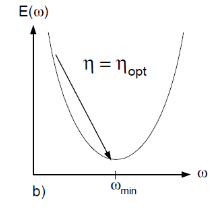
\includegraphics[width=10cm,height=5cm,keepaspectratio]{files/grad.png}
		\caption{Gradient Descent(\cite{lecun2012efficient})}
		\label{fig:act}
	\end{figure}
	This gives an optimized value, rather than the guaranteed value. Reaching the minima efficiently and in reasonable time is a very important research area. Convergence of gradient descent depends on many factors. Some of them are discussed here.\\
	\begin{figure}[H]
		\centering
		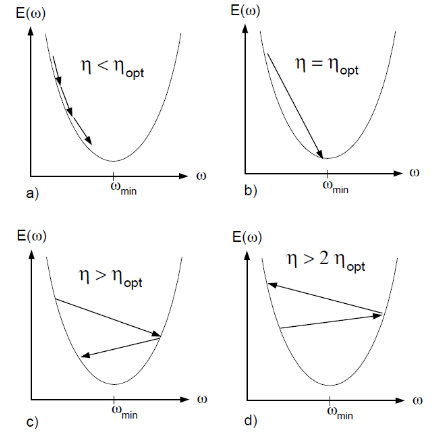
\includegraphics[width=10cm,height=15cm,keepaspectratio]{files/learningRate.png}
		\caption{Behavior for different learning rates (\cite{lecun2012efficient})}
		\label{fig:learn}
	\end{figure}
	\begin{itemize}
		\item Initialization of parameters is an important factor in determing how long the model takes to converge. Stochastic gradient descent applied to non-convex loss functions has no such convergence guarantee and hence the initial parameters should be chosen wisely for example initial parameters should be small and random values.
		\item Another factor is the how to choose the learning rate as discussed by \cite{lecun2012efficient}. Effects of choosing this factor is demonstrated in the fig, \ref{fig:learn}.
	\end{itemize}
	These techniques are important as convergence might be very slow and also sometimes lead to vanishing gradient or even exploding gradients. In such cases, clipping gradient, intelligent initialization of parameters, normalizing data and other tricks of trade makes life bit easier.
\end{enumerate}	
\section{\textit{n}-Gram Model}
There have been an increased research in Natural Language Processing which is mainly concerned with the interactions between computers and human languages. Both semantics and syntax of the language makes it understandable for humans. In language modeling, there has always been an active research for capturing both of these information. There are generally two types of \textit{n}-grams in Computational Linguistics.

\subsection{Word \textit{n}-grams}
This kind of \textit{n}-gram model is generally used in distributive word embeddings as they help in capturing semantic information in the language. These are particularly useful in learning words which are used in similar context. Variance in value of \textit{n} determines the quality of the model. 
\begin{center}
	\begin{tabular}{ c c }
		text:& to be or not to be\\
		Uni-gram:& to, be, or, not, to, be\\
		Bi-gram:& to\_be, be\_or, or\_not, not\_to, to\_be\\
		Tri-gram:& to\_be\_or, be\_or\_not, or\_not\_to, not\_to\_be\\
	\end{tabular}
\end{center}
\subsection{Character \textit{n}-grams}
The character \textit{n}-gram helps in capturing the morphological structure of the words. These are particularly helpful when dealing with morphological similar languages like Turkish or German. Therefore in such languages, one can say that the words are similar when they have a common root/morpheme. If we take the example of the English language, some of the words are formed by taking basic words and adding combinations of prefixes and suffixes to them. This can thus be considered as a good measure for similarity. 
\textit{n}-Gram is one approach to measure similarity between words  based on the common n-grams present in a word. Here \textit{n} can be 2,3,4. It algorithmically quantify the similarity between a set of strings from a finite alphabet. 
\begin{center}
	\begin{tabular}{ c c }
		text:& ankit\\
		Uni-gram:& a, n, k, i, t\\
		Bi-gram:&  \_a, an, nk, ki, it, t\_ \\
		Tri-gram:& \_an, ank, nki, kit, it\_ \\
	\end{tabular}
\end{center}
From some previous works, it can be deduced that \textit{n = 3, 4} gives the best results statistically. Example: The similarity between words "Minimal", "Minimize" is greater than the similarity between "Minimal" and "Maximize".\\
There has been a lot of work done in finding similarity between words using \textit{N}-Gram. \cite{kondrak2005n} has give a formal, recursive definitions of n-gram similarity and distance of the words. He has also proposed an efficient algorithms for computing them. The algorithm involves combining different similarities values obtained from different \textit{n}-gram models. 
We can thus select different values of \textit{n} for finding similarities based on the purpose. Uni-gram, bi-gram, tri-gram are some of the examples. One important consideration  that should be taken in account while calculating similarity is that spaces before the starting of the word and at the end of the word should also be taken in the set of \textit{n}-grams.\\
\\
\textbf{String Kernel Similarity}
One important use of \textit{n}-gram, is in computing string similarity as discussed in \cite{martins2006string} and \cite{bauc}.  In this work, we have also used \textit{n}-grams to calculate the \textit{String Kernel function}.\\
For example: If $s_1$ and $s_2$ are two words and $B_1$ and $B_2$ are their respective \textit{n}-gram sets then, a similarity function, $\mathcal{S}$, can be defined in equation, \ref{eq:sks}:\\
\begin{equation}\label{eq:sks}
\mathcal{S}(s_1,s_2) = \frac{2\times\mid B_1\cap B_2\mid}{\mid B_1 \mid + \mid B_2 \mid}
\end{equation}
and
\begin{equation}
d(s_1,s_2) = 1- \mathcal{S}(s_1,s_2)
\end{equation}
Here $d(s_1,s_2)$ can be seen as a distance measure between two words $s_1$ and $s_2$. This distance measure can then be used in a Kernel function. An example of such a kernel function is:
\begin{equation}
k(s_1,s_2) = exp\Bigg(\dfrac{-d^2(s_1,s_2)}{2\sigma^2}\Bigg)
\end{equation}
\section{Numeric Representation of Words}

\subsection{One Hot Vector Encoding}
For a vocabulary of size $\mathbf{V}$, one hot vector encoding helps in formalizing a vector of a word with the position of the word in the dictionary. Therefore a one hot vector of a word will have all "0" and at the position of the word in the dictionary, it will have a "1". The vector size is thus same as the size of vocabulary.
One hot vector encoding can also be seen as a hashing technique. This is illustrated in the following example.
\begin{center}
	For  the sentence \texttt{"the cat sat on the mat"}, one hot vector matrix will be represented as follows:
\end{center}
\begin{center}
	The dictionary of the sentence is:\\
	\{'the':0,'cat':1,'sat':2,'on':3,'mat':4\}\\
\end{center}
\begin{center}
	$\left(
	\begin{array}{ll}
	\text{the} \\
	\text{cat} \\
	\text{sat} \\
	\text{on}  \\ 
	\text{the}  \\ 
	\text{mat}  \\ 
	\end{array}%
	\right). = 
	\left( 
	\begin{array}{ll}
	\text{1 0 0 0 0} \\
	\text{0 1 0 0 0} \\
	\text{0 0 1 0 0} \\
	\text{0 0 0 1 0}  \\ 
	\text{1 0 0 0 0}  \\ 
	\text{0 0 0 0 1}  \\
	\end{array}%
	\right). $
\end{center}
As it can be inferred from the above example, such vectors only encode the information of the position of the word in the vocabulary and hence are very sparse. Such vectors are very less informative which becomes a limitation of this representation.
\subsection{Distributed Representations of Words: Word Embeddings}
To overcome the limitations of \texttt{one-hot vector}, a more informative representation is needed which can encode the information like semantic or syntactic similarities between the words. A distributed representation of words fulfills these requirements. These embeddings are captured using a "one hidden layer network architecture", such as \texttt{Continuous Bag Of Words (CBOW)} and \texttt{Continuous Skip Gram Model}.
\subsubsection{Continuous Skip Gram Model (CBOW Model)}
The model of Continuous Bag-of-Words Model(CBOW) is represented in the figure, \ref{fig:cbow_sg}. It follows a very similar approach as the feed forward NNLM proposed by \cite{bengio2003neural}. The goal of CBOW is to predict a word given a set of its context words. Context here is defined as the number of words to the left and to the right of the given word. Example of input and output with \textbf{C=1} of the model is demonstrated in the below example:\\
\textbf{Text:} \texttt{Roberta ran rings around Roman ruins.}\\
\textbf{Input and Output pair:}\\
 \texttt{(ran,[Roberta,rings]),(rings,[ran, around]), (around,[rings, Roman]),(Roman)
 	[around, ruins])...}
\begin{figure}[H]
	\centering
	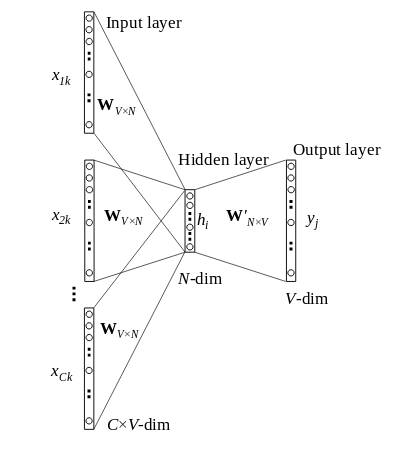
\includegraphics[width=15cm,height=12cm,keepaspectratio]{files/cbow.png}
	\caption{\textit{CBOW Model} (\cite{DBLP:journals/corr/Rong14})}
	\label{fig:cbow_sg}
\end{figure}
The model is a neural network with one hidden layer and consists of two weight matrices, $\mathbf{W_{V\times N}}$ and $\mathbf{W'_{N\times V}}$. These weights represents \textit{input word vectors}, $\mathbf{v}_w$ and \textit{output word vectors}, $\mathbf{v'}_w$. Since $\mathbf{x}$ are one-hot vector encoding for words, hence equation, \ref{eq:01} is essentially copying the corresponding row of $\mathbf{W}$ to $\mathbf{h}$. This implies that the activation function of the hidden layer units is linear. One important thing to note here is that the order of the words in context are averaged as presented in equation, equation \ref{eq:01} and hence the order of these words has no influence over the projection.
\begin{equation}\label{eq:01}
\begin{split}
\mathbf{h} & = \frac{1}{C} \mathbf{w}^T(\mathbf{x_1+x_2+...+x_C})\\
& = \frac{1}{C}(\mathbf{v}_{w_1}+\mathbf{v}_{w_2}+...+\mathbf{v}_{w_C})
\end{split}
\end{equation}
Each $\mathit{j^{th}}$, column in the matrix, $\mathbf{W'}$, of dimension ($N\times V$), is represented by the vector, $\mathbf{v'}_{w_{j}}$. This vector helps in calculating a score $\mathit{u_j}$ for each word in the vocabulary. This score is represented as:
\begin{equation}
\mathit{u_j} = \mathbf{v'}_{w_{j}}^{\mathbf{T}}\mathbf{h}
\end{equation}
This score can be used in a softmax classification model, to obtain the posterior distribution of words.
\begin{equation}
\mathit{y_j} = \mathit{p(w_j \mid w_{I,1}..w_{I,C})} = \dfrac{exp(u_j)}{\sum_{j'=1}^{V}exp(u_{j'})}
\end{equation}
This can be also represented by the following equation:
\begin{equation}\label{eq:02}
\mathit{p(w_j \mid w_{I,1}..w_{I,C})} =\dfrac{exp(\mathbf{v'}^T_{w_{j}} \mathbf{v}_{w_{I}})}{\sum_{j'=1}^{V}exp(\mathbf{v'}^T_{w_{j'}} \mathbf{v}_{w_{I}})}
\end{equation}
The model is thus trained by maximizing its log-likelihood on the training set or minimizing the negative log-likelihood of:
\begin{equation}
E = - \log p(w_j\mid w_{I,1},...,w_{I,C})
\end{equation}
The goal now is to optimize the weights so as to improve (in this case, maximize) the objective function in equation, \ref{eq:02}. This is done by deriving the gradient of the loss with respect to the embedding parameters/weights. An update to the embeddings is made by taking a small step in the direction of the gradient. When this process is repeated over the entire training set, this has the effect of moving the embedding vectors around for each word until the model is successful at discriminating real words from noisy words.
\subsubsection{Skip-Gram Model} 
Skip gram model is simpler model when compared to Continuous Bag of Words. It's goal is opposite of that of a CBOW model. In other words, at the output layer, instead of getting one multinomial distribution, there are $C$ multinomial distributions of the words. For example, using a window size of 1, we then have the dataset with context words one left and one right.\\
The dataset consists of a context and target pair. For example as shown below: \cite{tensorflow2015-whitepaper}:\\\\
\textbf{Text:} 
\texttt{Roberta ran rings around Roman ruins.}\\
\textbf{Input and Output pair:}
\texttt{([Roberta,rings], ran),([ran, around],rings), ([rings, Roman],around),([around, ruins],Roman)...}
\\\\
It is worth noting that larger the context window, \textbf{C}, more are training examples and thus can lead to a higher accuracy, at the expense of the training time.\\
\begin{figure}[H]
	\centering
	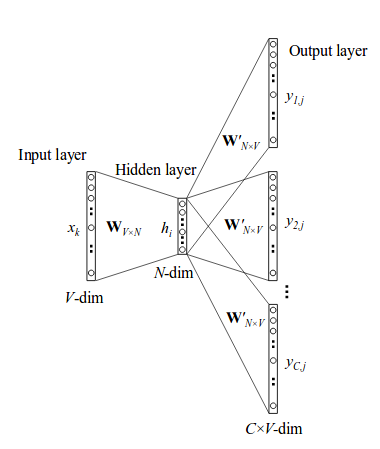
\includegraphics[width=15cm,height=12cm,keepaspectratio]{files/skip-gram.png}
	\caption{\textit{Skip-Gram Model} (\cite{DBLP:journals/corr/Rong14})}
	\label{fig:skip_sg}
\end{figure}
The scoring function remains same in this model as the CBOW model. Skip gram model performs better than the CBOW model, when it come across a rare word but is slower to train. This can be accounted to the fact that it does not average the embedding vectors. It seems like the model can learn better representations for the rare words when their vectors are not averaged with the other context words in the process of making the predictions.\\\\
In both the models, the quality of the word vectors increases significantly with amount of the training data. Both the models are widely popular because of their simple structure and use of a shallow network and have their own individual advantages. The skip gram model takes longer than CBOW model to get trained but performs much better on semantic tasks. Whereas CBOW model works better on syntactic tasks. The choice of the model depends on the problem domain and datasets.
\subsubsection{Optimizing Computational Efficiency}
In both the models proposed by \cite{mikolov2013efficient}, the output involves applying a \texttt{softmax function} represented in equation, \ref{eq:02}. If analyzed closely, it turns out to be computationally very expensive since the denominator of the \texttt{softmax function} is a dot product of the word with \textit{all the words in the vocabulary}. Thus there is a dire need for optimizing this function.
There are two approaches for optimizing the algorithms discussed above.
\begin{enumerate}
	\item \textbf{Hierarchical Softmax: }
	Hierarchical softmax, proposed by \cite{morin2005hierarchical}, is an approximation of softmax inspired by binary trees. It converts a flat softmax layer into a hierarchical layer that has the words as leaves and each node, explicitly represents the relative probabilities of its child nodes. Therefore, each word, $\textit{w}$ can be reached by an appropriate path from the root of the tree. The probability of a word, being the output word can be represented as:
	\begin{equation}
	p(w = w_O) = \prod_{j=1}^{L(w)-1} \sigma(\llbracket n(w,j+1) = ch(n(w,j))\rrbracket \cdot \mathbf{v'}^T_{n(w,j)}\mathbf{h})
	\end{equation}
	where:
	\begin{enumerate}
		\item $ch(n)$ is the left child of unit $n$.
		\item $\mathbf{v'}^T_{n(w,j)}$ is the vector representation of the inner units $n(w,j)$ .
		\item $\mathbf{h}$ is the output of the hidden layer.
		\item $\llbracket f\rrbracket$ is a special function which gives $1$ or$-1$ for condition being true or false. 
	\end{enumerate}
	The structure of the tree used by the hierarchical softmax has a considerable effect on the performance. \cite{mikolov2013distributed} used binary Huffman tree.
	\item \textbf{Negative Sampling: }
	Another optimization technique used in \cite{mikolov2013distributed} is negative sampling. The idea behind this approach is very straight forward when compared to hierarchical softmax. Essentially, the probability for selecting a word as a negative sample is related to its frequency, with more frequent words being more likely to be selected as negative samples. The Negative sampling (NEG) is defined by the objective function:
	\begin{equation}
	E = -\log \sigma(\mathbf{v'^T_{w_O}}\mathbf{h}) - \sum_{w \in \mathcal{W}_{neg}}\log\sigma(-\mathbf{v'}_{wj}\mathbf{h})
	\end{equation}
	where: 
	\begin{enumerate}
		\item $w_O$ is the output vector from the positive sample.
		\item $\mathcal{W}_{neg}$ are the negative sample set of words that are sampled from the noise distribution, $P_{n}(w)$ 
	\end{enumerate}
\end{enumerate}